\documentclass[border=3mm]{standalone}
\usepackage{amsmath,amssymb,pgfplots}
\usepgfplotslibrary{groupplots}
\pgfplotsset{compat=1.18}

\definecolor{evalteal}{HTML}{087F8C}
\definecolor{evalnavy}{HTML}{17324D}
\definecolor{evalgray}{HTML}{97A3B1}
\definecolor{evalorange}{HTML}{B95C16}

\begin{document}
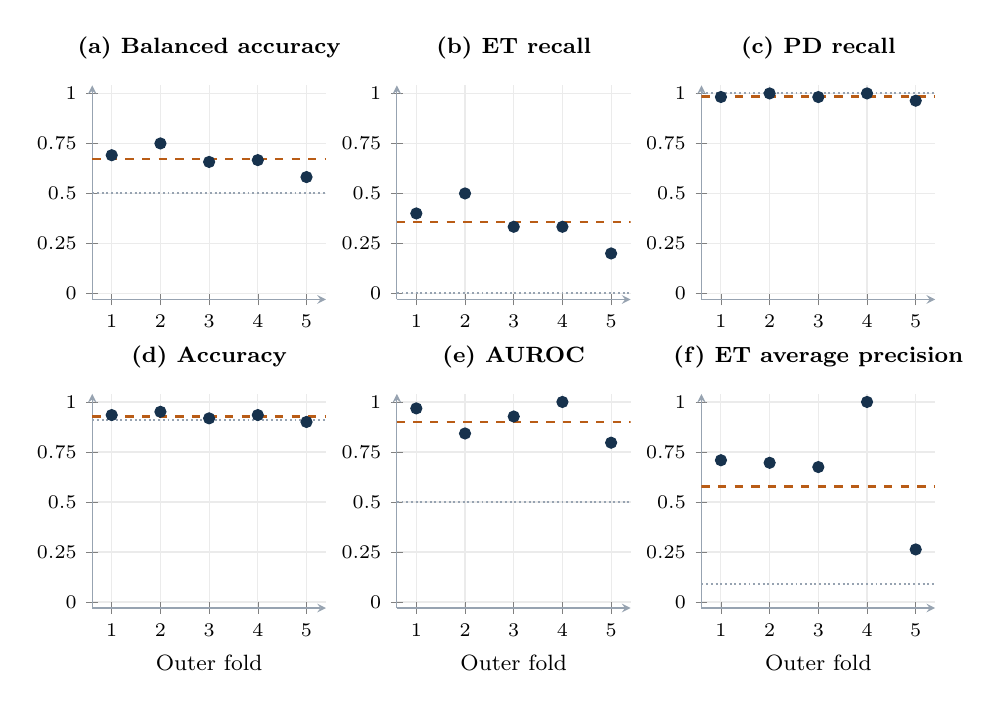
\begin{tikzpicture}
\begin{groupplot}[
 group style={group size=3 by 2,horizontal sep=0.9cm,vertical sep=1.2cm},
 width=4.55cm,height=4.3cm,xmin=0.6,xmax=5.4,ymin=-0.03,ymax=1.04,
 xtick={1,2,3,4,5},ytick={0,0.25,0.5,0.75,1},
 xlabel={Outer fold},axis lines=left,axis line style={evalgray},
 grid=major,grid style={black!8},
 tick label style={font=\scriptsize},label style={font=\footnotesize},
 title style={font=\footnotesize\bfseries},clip=true]
\nextgroupplot[title={(a) Balanced accuracy},xlabel={}]
\addplot[evalgray,densely dotted,line width=0.7pt] coordinates {(0.6,0.5) (5.4,0.5)};
\addplot[evalorange,dashed,line width=0.9pt] coordinates {(0.6,0.6713250518) (5.4,0.6713250518)};
\addplot[only marks,mark=*,mark size=2pt,evalnavy] coordinates {(1,0.6910714286) (2,0.75) (3,0.6575757576) (4,0.6666666667) (5,0.5818181818)};
\nextgroupplot[title={(b) ET recall},xlabel={}]
\addplot[evalgray,densely dotted,line width=0.7pt] coordinates {(0.6,0) (5.4,0)};
\addplot[evalorange,dashed,line width=0.9pt] coordinates {(0.6,0.3571428571) (5.4,0.3571428571)};
\addplot[only marks,mark=*,mark size=2pt,evalnavy] coordinates {(1,0.4) (2,0.5) (3,0.3333333333) (4,0.3333333333) (5,0.2)};
\nextgroupplot[title={(c) PD recall},xlabel={}]
\addplot[evalgray,densely dotted,line width=0.7pt] coordinates {(0.6,1) (5.4,1)};
\addplot[evalorange,dashed,line width=0.9pt] coordinates {(0.6,0.9855072464) (5.4,0.9855072464)};
\addplot[only marks,mark=*,mark size=2pt,evalnavy] coordinates {(1,0.9821428571) (2,1) (3,0.9818181818) (4,1) (5,0.9636363636)};
\nextgroupplot[title={(d) Accuracy}]
\addplot[evalgray,densely dotted,line width=0.7pt] coordinates {(0.6,0.9078947368) (5.4,0.9078947368)};
\addplot[evalorange,dashed,line width=0.9pt] coordinates {(0.6,0.9276315789) (5.4,0.9276315789)};
\addplot[only marks,mark=*,mark size=2pt,evalnavy] coordinates {(1,0.9344262295) (2,0.9508196721) (3,0.9180327869) (4,0.9344262295) (5,0.9)};
\nextgroupplot[title={(e) AUROC}]
\addplot[evalgray,densely dotted,line width=0.7pt] coordinates {(0.6,0.5) (5.4,0.5)};
\addplot[evalorange,dashed,line width=0.9pt] coordinates {(0.6,0.8999741201) (5.4,0.8999741201)};
\addplot[only marks,mark=*,mark size=2pt,evalnavy] coordinates {(1,0.9678571429) (2,0.8424242424) (3,0.9272727273) (4,1) (5,0.7963636364)};
\nextgroupplot[title={(f) ET average precision}]
\addplot[evalgray,densely dotted,line width=0.7pt] coordinates {(0.6,0.09210526316) (5.4,0.09210526316)};
\addplot[evalorange,dashed,line width=0.9pt] coordinates {(0.6,0.5776189524) (5.4,0.5776189524)};
\addplot[only marks,mark=*,mark size=2pt,evalnavy] coordinates {(1,0.7087301587) (2,0.6959259259) (3,0.6746031746) (4,1) (5,0.2627679567)};
\end{groupplot}
\end{tikzpicture}
\end{document}
